\documentclass{beamer}

\usetheme{Berlin}
\usecolortheme{beaver}

\usepackage{graphicx} 
\usepackage{booktabs} 

\title[Improving DLS]{Improving Duckworth-Lewis: Statistical Methods for Resetting Score Targets in Limited-Overs Cricket} 

\author{Matthew Knowles} 
\institute[UoY] 
{
University of York \\ 
\medskip
\textit{mk1320@york.ac.uk} 
}
\date{\today} 

\begin{document}

\begin{frame}
\titlepage 
\end{frame}

\begin{frame}
\frametitle{Plan for the Talk} 
\tableofcontents 
\end{frame}

\section{Background}
\begin{frame}
\frametitle{Cricket}

\begin{itemize}
    \item 2 teams of 11 players. One team bats, the other fields. \\
    \pause
    \item Score measured in runs. Aim: Score as many as you can before losing 10 wickets. \\
    \pause
    \item Focus in this project is limited overs cricket. Games last 50 overs, which takes about 3 hours.
\end{itemize}

\end{frame}

\begin{frame}
\frametitle{Setting the scene: The need for score resetting}

\begin{itemize}
    \item Cricket is very sensitive to external factors, such as rain and daylight. \\
    \pause
    \item If it gets too dark, the ball becomes very hard to see and so the game is stopped. \\
    \pause
    \item Similarly, if it rains, the game is stopped due to the adverse affect this has on the pitch. \\
\end{itemize}
    
\end{frame}

\begin{frame}
    \frametitle{A motivating example}
    \begin{itemize}
        \item To illustrate the issue, consider the following example. \\
        \pause
        \begin{example}
            Team A scores 320 runs in their 50 overs, losing 8 wickets in the process. While team B is batting, 
            it begins to rain, and the umpires call the game off with team B on 118-2 from 34 overs. After the rain stops,
            there is only time for 6 overs of play. 
        \end{example}
        \pause    
        \item Clearly, at this point it is unfair to expect team B to chase down 222 runs in 6 overs instead of the 16 they should 
            have had. So for this reason, score target adjustment is needed to keep the game fair, despite the loss of time.
\end{itemize}
        
\end{frame}

\begin{frame}
\frametitle{Duckworth, Lewis}

\begin{itemize}
    \item Statisticians Frank Duckworth and Tony Lewis set about a way to reduce score targets appropriately to overcome challenges
        like the one in the last example. \\
    \pause
    \item They introduce the following formula
        $$
            Z(u,w) =  Z_0(w)(1e^{-b(w)u})
        $$ 
        Which gives the runs scored with $u$ overs remaining and $w$ wickets lost. Note that the actual value of $Z_0$ and $b$, the decay constant are not given due to commercial agreements.
    \pause
    \item Consider the special case at the start of an N-over innings. I.e $u=N$ and $w=0$.
         $$
            Z(N,0) = Z_0(1 - e^{-bN})
        .$$

\end{itemize}

\end{frame}

\begin{frame}
    \frametitle{Duckworth and Lewis (Contd.)}
    \begin{itemize}
     \item We incorperate the above into a ratio that forms the basis of the Duckworth-Lewis method.
        $$
            P(u,w) = \frac{Z(u,w)}{Z(N,0)}
        .$$ 
    \pause
    \item Computing all values for $P$ with $1 \leq u \leq 50$ and $0 \leq w \leq 10$ gives a table of results.
        It is from this table that the revised score target is calculated. 
    \end{itemize}
\end{frame}

\begin{frame}
    \frametitle{Stern}
    \begin{itemize}
        \item With the introduction of an even shorter form of the game, ``Twenty20'', consisting of only 20 
            overs instead of 50. The method needed to be updated.
        \pause
        \item Steven Stern introduced updates in 2015 to account for the new increase in game scores. 
    \end{itemize}
\end{frame}


\begin{frame}
\frametitle{Problems with DLS}
    \begin{itemize}
        \item DLS has a tendancy to reset score targets that are unrealistic, and as such ruin the competetive 
            nature of a match
        \pause
        \item DLS does not account for fielding restrictions that are in place at different pooints in the game 
        \pause
        \item It is not easy to understand, especially for players and officials without any mathematical education
    \end{itemize}
\end{frame}

\section{Neural Networks in Cricket}
\begin{frame}
\frametitle{Structure of Neural Networks}
    \begin{itemize}
        \item Neural Networks are a mathematical model based on neurons in a brain
        \pause
        \item To artificially create such a model, we use a system of nodes and synapses
    \end{itemize}
    \begin{example}
        \centering
        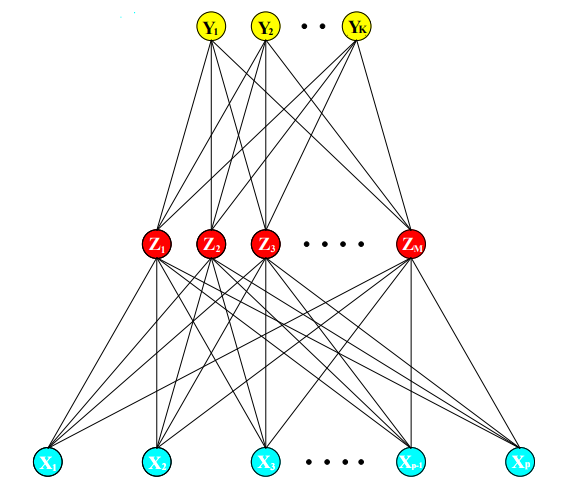
\includegraphics[scale=0.3]{../Thesis/figures/nn.png}
    \end{example}
\end{frame}

\begin{frame}
    \frametitle{Mathematically Representing Neural Networks}
    \begin{itemize}
    \pause
    \item Layers of nodes (perceptrons). $k$ ``hidden'' layers sandwiched by an input layer and an output layer. \\
    \pause
    \item Each node in layer j connects to each node in layer $j+1$. Connection is defined by a weight and a bias.  \\
    \pause
    \item Let the layer $k_i$ have m nodes, and the layer $k_i+1$ have n nodes. Then the weights between the layers are given by the matrix
    \pause
    \begin{equation}
        W =
        \left[ {\begin{array}{cccc}
          w_{1,1} & w_{1,2} & \cdots & w_{1,m}\\
          w_{2,1} & w_{2,2} & \cdots & w_{2n}\\
          \vdots & \vdots & \ddots & \vdots\\
          w_{n,1} & w_{n,2} & \cdots & w_{n,m}\\
        \end{array} } \right]
        \label{weights1}
    \end{equation}
\end{itemize}
\end{frame}
    

\begin{frame}
    \frametitle{Mathematically Representing Neural Networks (contd)}
    \begin{itemize} 
    \item The values of the nodes in layer $k+1$, denoted $A_{(k+1)}$ is given by the matrix equation $A_{(k+1)} = \sigma(WA_{(k)}+b_{(k)})$. Where
        b is the vector containing the biases, and $\sigma()$ is the \textit{activation function}.
    \pause
\item The choice of activation function is pretty much problem dependent, and depends a little bit on the data. In our case, we used the sigmoid activation function $\sigma : \mathbb{R} \rightarrow \mathbb{R}$ defined by  $\sigma(x) = (1+\exp(-x))^{-1}$.
    \end{itemize}
\end{frame}

\begin{frame}
    \frametitle{How do Neural Networks ``learn''?}
    \begin{itemize}
        \item The idea of learning comes from updating the weights and biases to reduce the error made when predicting a result.
        \pause
        \item We start by initialising values of weights, biases, activation values by drawing random samples from a distribution. 
        \pause
        \item We pass training data through the network, and see what the output is. By comparing this output to the actual value for that piece of data, we get an error value. 
        \pause
        \item We then employ the backpropogation algorithm to readjust the values of the weights and biases in accordance with the 
            error. This looks to find a set of weights and biases that give the least error on the training data.
    \end{itemize}
\end{frame}

\begin{frame}
    \frametitle{The Run-Rate Network}
    \begin{figure}
        \centering
        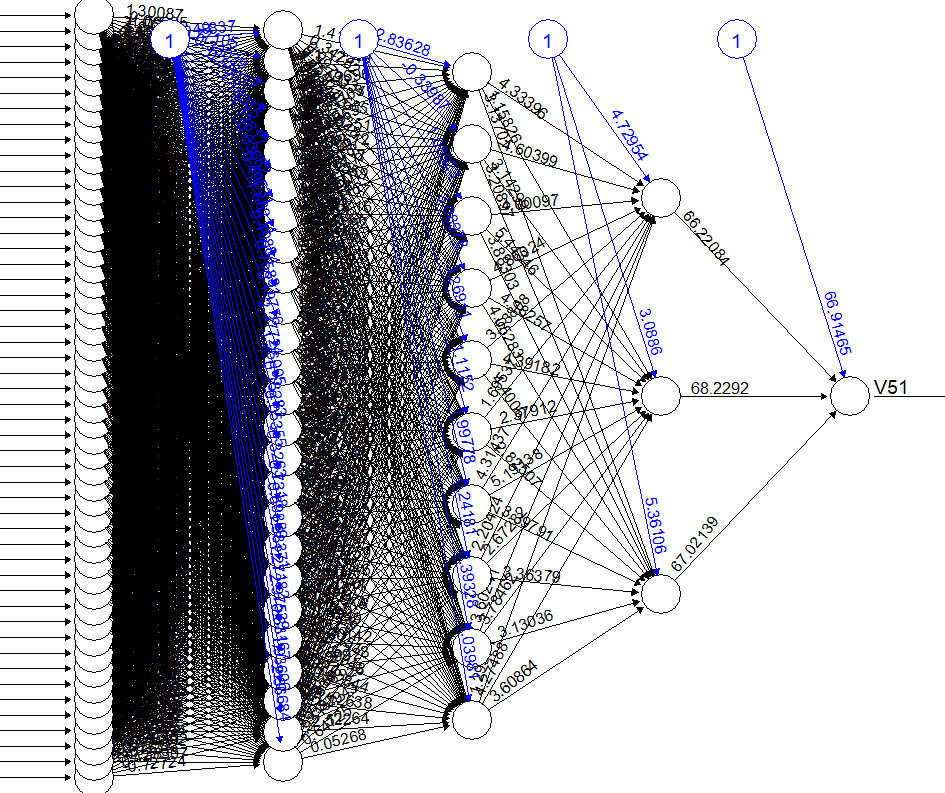
\includegraphics[scale=0.2]{../Thesis/figures/net.png}
    \end{figure} 
\end{frame}

\section{Resetting Score Targets}
\begin{frame}
    \frametitle{Different Scenarios}
\begin{itemize}
    \item Since the aim is to reset score targets when a full innings cannot be played, we have the issue 
        of having 50 inputs to the network. There are two examples of how we could fix this. 
    \pause
\end{itemize}
    \begin{example}
        Assume 35 overs of play have occured. Leaving 15 overs without data.
        \begin{enumerate}
            \item Assert a value of 0 on the remaining overs and see what the network predicts
            \item Draw random values based on historical perfomance of teams in the remaining overs
        \end{enumerate}
    \end{example}
\end{frame}

\begin{frame}
    \frametitle{Different Scenarios (contd)}
    \begin{itemize}
        \item  To test which method worked better, we took a test data set, and tested which option worked better. 
        \pause
        \item As it turns out, trying to fill in the gaps, didn't work at all. The predictions were way off and 
            the corrolation between predicted results and actual results was almost 0.
        \pause
        \item Leaving the unplayed overs blank was much more successfull, and had a corrolation of 0.49. So not great,
            but much better.
    \end{itemize}  
\end{frame}

\begin{frame}
    \frametitle{World Cup Simulation Study}
    \begin{itemize}
        \item To test the method fully, we took the 3 games from the 2019 world cup that used DLS to decide a result, 
            and used our method instead. 
        \pause
        \item Of the 3 games, only 1 had the result changed, which meant the final standings of the tournament were
            virtually unchanged, except Bangladesh finish above South Africa for $7^{th}$ place. 
        \pause
        \item The key difference was in the scores set, the score targets were far more attianable by the batting team,
            which would have lead to a more competative set of games. The India vs Pakistan game was ruined by DLS in this 
            way. Since they needed 27.2 an over at one point. 
    \end{itemize}
\end{frame}

\section{Conclusions}

\begin{frame}
    \frametitle{Did we improve DLS?}
    \begin{itemize}
        \item Not really. Aside from giving slightly more competative score targets, the method was still lacking. 
        \pause
        \item From an entertainment point of view, this method is better, but from a pure cricket perspective, 
            DLS is still more reliable
        \pause 
        \item With more data, this method will become more reliable in the future, but this is constrained by
            the number of cricket games played each year.
    \end{itemize}
\end{frame}

\begin{frame}
\Huge{\centerline{Any Questions?}}
\end{frame}


\end{document} 
